% !TEX root=./chap-04.tex
%-----全局定义-----
\documentclass[type=doctor]{fduthesis}
% \usepackage{fdudoc}

%-----FDU thesis setup-----
\fdusetup{
    style = {
        font = libertinus,
        cjk-font = founder,
        font-size = -4,
        fullwidth-stop = mapping,
        % footnote-style = xits,
        hyperlink = color,
        hyperlink-color = default,
        bib-backend = bibtex,
        bib-resource = {../thesis.bib},
        % bib-style = achemso,
        % cite-style = numerical,
        % declaration-page = {declaration.pdf},
        % 插入扫描版的声明页 PDF 文档
        % 默认使用预定义的声明页,但不带签名
        auto-make-cover = false,
        % 是否自动生成论文封面(封一)、指导小组成员名单(封二)和声明页(封三)
        % 除非特殊需要(e.g. 不要封面),否则不建议设为 false
    },
    %
    % info 类用于录入论文信息
    info = {
    title = {双杂化密度泛函分子能量与性质\\计算方法进展与测评},
    title* = {
        Recent Progress on Computational Method and Benchmark
        on Molecular Energy and Property of Doubly Hybrid Functional Approximations},
    % 英文标题
    %
    author = {祝震予},
    supervisor = {徐\quad 昕\quad 教授},
    major = {物理化学},
    degree = academic,
    department = {化学系},
    student-id = {17110220038},
    % date = {2023 年 1 月 1 日},
    % 日期
    % 注释掉表示使用编译日期
    instructors = {
        { 徐 昕    教 授 },
        { 张 颖    教 授 },
        { 段 赛   青年研究员},
        { 郑 晓    教 授 },
    },
    % 指导小组成员
    % 使用英文逗号 “,” 分隔
    % 如有需要,可以用 \quad 手工对齐
    %
    keywords = {密度泛函理论, 双杂化泛函, 电子云密度, 解析梯度性质, 静态极化率},
    % 中文关键词
    % 使用英文逗号 “,” 分隔
    %
    keywords* = {density functional theory, doubly hybrid functional, electron density, analytical derivative property, static polarizability},
    % 英文关键词
    % 使用英文逗号 “,” 分隔
    %
    clc = {O641.12},
    % 中图分类号
    }
}

%-----fduthesis issues-----
% issue #86
\ExplSyntaxOn
\tl_set:Nn \c__fdu_cover_info_align_tl { c @ { \c__fdu_fwid_colon_tl } l }
\ExplSyntaxOff
% 化学系图表格式要求
\ExplSyntaxOn
\cs_set:Npn \thefigure
{ \thechapter . \__fdu_arabic:n { figure } }
\cs_set:Npn \thetable
{ \thechapter . \__fdu_arabic:n { table } }
\ExplSyntaxOff

% expl3 在 tabulararray 包的冲突
% https://tex.stackexchange.com/a/463283
\usepackage{expl3}
\ExplSyntaxOn
\int_new:N \g__tblr_defined_hdash_styles_prop
\int_new:N \g__tblr_defined_vdash_styles_prop
\int_new:N \g__tblr_initial_rows_prop
\int_new:N \g__tblr_initial_columns_prop
\int_new:N \g__tblr_initial_table_prop
\int_new:N \g__tblr_initial_cells_prop
\int_new:N \g__tblr_initial_hlines_prop
\int_new:N \g__tblr_initial_vlines_prop
\ExplSyntaxOff

%-----图表设置-----
\usepackage{siunitx}
\usepackage{enumitem}
\newcommand{\tabnote}[1]{\textsuperscript{\emph{#1}}}
\usepackage{threeparttable}
\usepackage{threeparttablex}
\usepackage{graphicx}
\usepackage{longtable}
\usepackage{longfigure}
\usepackage{subcaption}
\usepackage{float}
\usepackage{lscape}
\usepackage{multicol}
\usepackage{multirow}
\usepackage{arydshln}
\usepackage{dcolumn}
\newcolumntype{d}[1]{D{.}{.}{#1}}
\setlength\dashlinedash{0.5pt}
\setlength\dashlinegap{1.5pt}
\setlength\arrayrulewidth{0.5pt}
\usepackage[figuresright]{rotating}
% \usepackage{booktabs}
\usepackage{tabularray}
\UseTblrLibrary{booktabs}
\usepackage{tcolorbox}

%-----化学符号-----
\usepackage[version=4]{mhchem}

%-----数学记号----
\usepackage[ntheorem]{empheq}
\allowdisplaybreaks[1]

%-----其它定义-----
\definecolor{msblue}{rgb}{0.05859375,0.28515625,0.43359375}
\definecolor{msorge}{rgb}{0.75390625,0.35156250,0.08593750}
\usepackage{ifthen}
\newcommand{\Schrodinger}{Schr\"o\-dinger}
\usepackage{tikz}
\usetikzlibrary{arrows.meta, graphs, shapes.misc, positioning}

% tablenotes 与表格内注释超链接 (from fdudoc.cls)
\makeatletter
\renewlist{tablenotes}{description}{1}
\setlist[tablenotes]{
  format      = \normalfont\itshape\tnote@item,
  labelwidth  = 0.5em,
  itemindent  = 0pt,
  rightmargin = \tabcolsep,
  leftmargin  = \the\dimexpr\tabcolsep+1em\relax,
  after       = \@noparlisttrue}
\AtBeginEnvironment{tablenotes}{%
  \setlength\parindent{2\ccwd}%
  \normalfont\footnotesize}
\AtBeginEnvironment{threeparttable}{%
  \stepcounter{tpt@id}%
  \edef\curr@tpt@id{tpt@\arabic{tpt@id}}}
\newcounter{tpt@id}
\def\tnote@item#1{%
  \Hy@raisedlink{\hyper@anchor{\curr@tpt@id-#1}}#1}
\def\TPTtagStyle#1{\textit{\hyperlink{\curr@tpt@id-#1}{#1}}}
\makeatother

% 用于表格注释与 threeparttable 环境引入的便利函数
\renewcommand{\TPTminimum}{\linewidth}
\newcommand{\widetabular}[2]{%
\ifx&#2&
  \begin{threeparttable}
    \centerline{\makebox[2\linewidth]{#1}}
  \end{threeparttable}
\else
  \begin{threeparttable}
    \centerline{\makebox[2\linewidth]{#1}}
  \begin{tablenotes}[nosep, topsep=0.5em]
    #2
  \end{tablenotes}
  \end{threeparttable}
\fi}

% 用于分章节编译与统稿的代码
\newcommand{\alert}[1]{{\color{red}{#1}}}
\newcommand{\alertref}[1]{{\color{red}{#1}}}
\newcommand{\alerthyperref}[2]{{\color{red}{#2}}}
\newcommand{\blindproof}[1]{{\color{blue}{#1}}}

% 用于表示方法的格式
\newcommand{\textmt}[1]{\textsf{#1}}

% 向量加粗的简记
\newcommand{\bm}{\symbfit}

% 保证 mathbb 被花括号包含
\renewcommand{\mathbb}[1]{{\symbb{#1}}}

%---------设定区结束----------

% 格式检查列表
% [ ] 表格数据使用 \widetabular{}{} 插入,以替代自定义的 \tabnote 和默认的 threeparttable。
% [ ] 表格 caption 在上,图片 caption 在下。图片不引入注释。
% [ ] 表格尽可能不引入纵向分割线。
% [ ] 建构术语表与符号表,避免文中出现术语定义、特别是英文定义。


\begin{document}

%---------预定设置区----------
\title{\textbf{双杂化密度泛函分子能量与性质计算方法的测评与进展\\第四章草稿}}
\author{祝震予}
\maketitle
\vspace{-10pt}

\tableofcontents

%---------正  文  区----------

\setcounter{section}{3}

\section{双杂化泛函原子体系电子云密度与能量测评}

\subsection{引言}

DFT (密度泛函理论) 在 Hohenberg-Kohn 定理\cite{Hohenberg-Kohn.PR.1964}的框架下,是原理上严格的理论;即没有引入任何近似,且必然存在一个对所有体系普适的、严格正确的泛函 $F[\rho]$;它可以导出精确的能量、电子云密度、各种分子或物质性质、以至于精确的波函数本身。

但现实是,我们难以获得严格的密度泛函本身。依 Levy 的设想\cite{Levy-Levy.PNAS.1979},真实泛函需要在完整的波函数空间下作搜索,其代价是巨大的。更晚的讨论表明,所有 $k$-local Hamiltonian 问题 ($k > 2$) 与 $N$ 可表示问题是 QMA 的 (量子计算机下非多项式的、困难的)\cite{Kempe-Regev.SJC.2006, Liu-Verstraete.PRL.2007};进而 DFT 问题也是 QMA 的\cite{Schuch-Verstraete.NP.2009}。具体来说,普适泛函的计算消耗、泛函变量的空间两者总存在其一是 QMA 问题:
\begin{itemize}[nosep]
    \item 使用波函数 $\Psi$ 作为基本变量,而不用密度 $\rho(\bm{r})$ 描述;则由于过大的变量空间,计算消耗是 QMA 的 (Full-CI、QMC 或 Levy 约束搜索);
    \item 电子云密度 $\rho(\bm{r})$ 作为变量,则普适泛函 $F[\rho]$ 的计算消耗是 QMA 的;所有对 $F[\rho]$ 计算消耗将至 P (多项式复杂度) 的尝试都必然是近似 (DFT 理论);
    \item 若不使用单粒子密度 $\rho(\bm{r})$ 而使用双粒子密度 $\rho_2(\bm{r}, \bm{r}')$ 构造泛函,那么即使 $F[\rho_2]$ 的计算复杂度可能降至 P;但为限制双粒子密度 $\rho_2 (\bm{r}, \bm{r}')$ 在其定义域 ($N$ 可表示空间),其代价仍然是 QMA 的 (2-RDM 框架)。
\end{itemize}
因此,任何理论或实现框架都无法简单地解决分子或物质模拟问题。

但从具体实现上,DFT 理论近似的普适泛函 $F[\rho]$ 计算消耗小、且 $\rho(\bm{r})$ 作为变量的空间小,从而广受物质计算工作者的欢迎。而跨越构造普适泛函 $F[\rho]$ 的困难,则成为泛函开发者不懈的追求。

但在如何克服 $F[\rho]$ 构造上的困难,对其作有效的近似,不同的研究者持有不同的态度。一些研究者坚持对 $F[\rho]$ 的形式与性质作深入的研究;若了解愈多 $F[\rho]$ 的严格性质 (exact constraints),就愈接近真实的严格普适泛函\cite{Kohn-Sham.PR.1965, Slater-Slater.PR.1951, Vosko-Nusair.CJP.1980, Perdew-Ernzerhof.PRL.1996, Adamo-Barone.JCP.1999, Ernzerhof-Scuseria.JCP.1999, Tao-Scuseria.PRL.2003, Cohen-Yang.CR.2012, Su-Xu.JCP.2014, Sun-Perdew.PRL.2015, Medvedev-Lyssenko.S.2017}。
另一些研究者在承认可预见的未来内 $F[\rho]$ 难以精确地构造的基础上,着重于更准确地描述具体的、当前物质科学所关心的问题;愈多类型的体系与性质可以被精确地描述,就愈接近真实的严格普适泛函\cite{Becke-Becke.PRA.1988, Lee-Parr.PRB.1988, Becke-Becke.JCP.1993, Zhao-Truhlar.JCP.2006, Grimme-Grimme.JCP.2006, Zhao-Truhlar.TCA.2008, Zhang-Goddard.PNAS.2009, Chai-Head-Gordon.JCP.2009, Zhang-Goddard.PNAS.2011, Zhang-Xu.JCP.2012, Yu-Truhlar.JCP.2016, Chen-Weinan.JCTC.2021}。

表面上,这两种看法的差异在于构造 $F[\rho]$ 时,是否存在经验参数。一般来说,前者通过严格性质构造 $F[\rho]$ 的途径,会使用较少甚至于没有经验参数。后者则通常对 $F[\rho]$ 作参数化;针对其所关心的物质计算问题,拟定数据训练集与验证集,对参数化的 $F[\rho]$ 作监督学习。而从实践的经验上,对于经验参数拟合的泛函,若计算问题处在训练集或验证集中,则通常有优异的表现;但若超出这些数据集的范围,则其表现很有可能因过拟合现象而粗强人意。相比之下,非经验参数拟合的泛函更有可能在各种物质及其性质上有良好的表现。

目前常用的密度泛函近似中,大多数都带有经验参数;而这些经验参数通常是针对能量性质的数据集而优化的。Medvedev 等\cite{Medvedev-Lyssenko.S.2017}指出,目前绝大多数泛函开发者关注于更精确地描述物质能量;其中不乏声音认为对能量更好的描述,可以给出更精确地泛函。但另一方面,电子云密度 $\rho(\bm{r})$ 作为密度泛函 $F[\rho]$ 的参量,作为连接多电子体系与能量的关键桥梁,却很少被关注到。基于对轻原子与正离子体系的电子云密度系统性的分析与测评,Medvedev 等认为,依泛函提出的年代顺序,2000 年以前发展的泛函在电子云密度上的表现较好、表现出 DFT 理论与其近似的进步;但 2000 年以后发展的泛函中,一部分泛函由于物理上不满足严格的性质、以及过分宽松的多经验参数拟合,使得后来的泛函在电子云密度的总体表现上逐年次第劣化。注意到密度泛函近似的目标是逼近普适泛函,而普适泛函应当能对所有的物质性质作精确的模拟;电子云密度作为密度泛函的重要物理量,当然并不例外。因此,对于这部分泛函,Medvedev 等人无法认同它们正在逼近普适泛函的道路上。同时他们认为,对于非参数或少量经验参数拟合的另一部分泛函,电子云密度确实地随“Jacob 阶梯”\cite{Perdew-Schmidt.ACP.2001}的爬升而愈加精确。

对于 Medvedev 等人的工作,不同的研究者表达过不同的看法。在 Kepp 的评论\cite{Kepp-Kepp.S.2017}中,其中一个重要的着眼点是,$F[\rho]$ (或者引入外势后的 $E[\rho]$) 作为泛函,它是 $\rho(\bm{r})$ 作为宗量、到能量值作为应变量的映射;只有两者都能描述好,近似的泛函才能认为真正地走在正确的道路上。同时,Kepp\cite{Kepp-Kepp.S.2017} 与王颖等人\cite{Wang-He.JCTC.2017} 对评价标准,特别关于涉及 $\nabla^2 \rho(\bm{r})$ 的径向函数 LR 与基组选取的问题上有针对性的深入研究。

而对于双杂化泛函,特别是 XYG3 型泛函 (xDH 型泛函)\cite{Zhang-Goddard.PNAS.2009},其一方面在“Jacob 阶梯”的顶端,原则上通过这些信息可以精确的描述真实泛函的性质。它同时包含非局域交换 (严格交换能) 与相关效应 (以 MP2 型相关能为典型);其基于 G\"orling-Levy 二阶微扰\cite{Goerling-Levy.PRB.1993, Goerling-Levy.PRA.1994}、且 xDH 型泛函在自洽场与能量两步计算都使用了包含完整的相关与交换信息,理论上有可靠的依据。另一方面,多数双杂化泛函含有少量的经验参数;这既能保证泛函在化学关心的问题上有良好的表现,但同时也不会轻易地过度拟合,而破坏泛函在训练集外的表现、以及对理论发展的偏离。因此我们期待,以 xDH 型泛函为代表的双杂化泛函,在除能量以外的其他训练集所没有涵盖到的性质上,也可能有良好的表现。

在本章与第六章,我们将对上述猜测作验证。我们基于 Medvedev 等人的工作\cite{Medvedev-Lyssenko.S.2017},对双杂化泛函作较为系统地评测。我们将同时关注能量 $E$ 与密度 $\rho(\bm{r})$ 的表现,并对基组依赖性作简要的讨论。我们期望表明,双杂化泛函不仅在反应能量上有良好的表现\cite{Su-Xu.WCMS.2016, Goerigk-Grimme.PCCP.2017, Zhang-Xu.JPCL.2021, Santra-Martin.JPCL.2021};在原子体系的电离和电子云密度的表现上,也沿着“Jacob 阶梯”仍然走在正确的道路上。

\subsection{实现细节}

\subsubsection{计算体系与方法}

本工作所涉及的体系是 14 个原子或离子体系 (\ce{Be^0}, \ce{B^+}, \ce{B^3+}, \ce{C^2+}, \ce{C^4+}, \ce{N^3+}, \ce{N^5+}, \ce{O^4+}, \ce{O^6+}, \ce{F^5+}, \ce{F^7+}, \ce{Ne^0}, \ce{Ne^6+}, \ce{Ne^8+}) 的电子云密度与能量。这些体系均为 2 ($1s^2$)、4 ($1s^2 2s^2$)、10 ($1s^2 2s^2 2p^6$) 电子体系。

与 Medvedev 等人的工作\cite{Medvedev-Lyssenko.S.2017}一致地,对于非变分方法,电子云密度 $\rho (\bm{r})$ 均使用弛豫密度生成 (对于 xDH 型泛函弛豫密度以 $D_{\mu \nu}^\textsf{PT2}$ 表示\alert{第三章公式})。测评过程所选用的基组是 aug-cc-p$\omega$CV5Z\cite{Dunning-Dunning.JCP.1989, Kendall-Harrison.JCP.1992, Peterson-Dunning.JCP.2002};对于使用到 RI 近似的情形,其辅助基组使用 PySCF 默认的自动生成方案\cite{Stoychev-Neese.JCTC.2017}。所有双杂化密度泛函选用经 PySCF 默认简化的 (120, 770) 格点积分,测评所用程序为 PySCF (2.4.0)\cite{Sun-Chan.WCMS.2018, Sun-Chan.JCP.2020} 与 dh (commit 80ca9e8)。本工作中涉及到的 post-HF 方法计算使用 Gaussian 09\cite{Gaussian09} 实现。

本工作也会对基组依赖性、RI 近似精度等问题作讨论;其具体的计算方法将在具体的讨论中展开。

本工作早期通过本地修改的 NWChem\cite{Valiev-Jong.CPC.2010}与 Multiwfn\cite{Lu-Chen.JCC.2012}实现。

\subsubsection{径向函数与密度测评标准定义}

本工作所采用的测评标准与 Medvedev 等人的工作\cite{Medvedev-Lyssenko.S.2017}一致,通过分析密度格点的径向分布函数 (RDF, \underline{R}adial \underline{D}istribution \underline{F}unction) 以作评测。该 RDF 的坐标选取为以原子核为中心均匀分布的 0 -- 10 \AA 的 50000 个格点。

在特定密度矩阵 $D_{\mu \nu}$ 下,电子云密度 $\rho(\bm{r})$ 定义为
\begin{equation}
    \rho(\bm{r}) = \sum_{\mu \nu} D_{\mu \nu} \phi_{\mu} (\bm{r}) \phi_{\nu} (\bm{r})
\end{equation}
对于原子体系,上述函数仅与电子到原子核距离 $r$ 有关,因此上述密度也写为 $\rho(r)$。密度径向函数 RHO、梯度 GRD 与二阶梯度 LR 分别定义为
\begin{align}
    \text{RHO}(r) &= 4 \pi r^2 \rho(r) \\
    \text{GRD}(r) &= 4 \pi r^2 | \nabla \rho(r) | = 4 \pi r^2 \left| \frac{\partial \rho(r)}{\partial r} \right| \\
    \text{LR}(r) &= 4 \pi r^2 \nabla^2 \rho(r) = 4 \pi r^2 \frac{\partial^2 \rho(r)}{\partial r^2}
\end{align}
对于给定的性质 $P \in \{\text{RHO}, \text{GRD}, \text{LR}\}$、原子或离子 $a \in \{\ce{Be^0}, \ce{B^+}, \cdots, \ce{Ne^8+}\}$、以及泛函近似或 post-HF 方法 $f, g$,RMSD (\underline{R}oot-\underline{M}ean \underline{S}quared \underline{D}eviation) 误差定义为
\begin{equation}
    \text{RMSD}_{P, a, (f, g)} = \sqrt{\frac{1}{N} \sum_i^N \big(P_{a, f} (r_i) - P_{a, g} (r_i) \big)^2}
\end{equation}
其中 $N = 50000$ 为格点数。特别地,若 $g = \textsf{CCSD}$,则简记 $\text{RMSD}_{P, a, f} = \text{RMSD}_{P, a, (f, \textsf{CCSD})}$。为了合理地将不同性质的误差作公平的对比,上述的 RMSD 误差将除以性质均值数 median RMSD,得到 MNAE (\underline{M}edian-\underline{N}ormalized \underline{A}bsolute \underline{E}rror):
\begin{equation}
    \text{MNAE}_{P, a, (f, g)} = \frac{\text{RMSD}_{P, a, (f, g)}}{\text{median}_{P} \text{RMSD}_{P, a, (f, g)}}
\end{equation}
最后,通过对原子指标 $a$ 求取极大值或平均值,可以得到泛函或方法 $f$ 在性质 $P$ 上的表现:
\begin{align}
    \text{maxMNAE}_{P, (f, g)} &= \max_a \text{MNAE}_{P, a, (f, g)} \\
    \text{meanMNAE}_{P, (f, g)} &= \underset{a}{\text{mean}} \, \text{MNAE}_{P, a, (f, g)}
\end{align}

本工作的 median RMSD,对于 RHO (单位 $\text{e} \, \text{\AA}^{-1}$) 为 0.009943368,对于 GRD (单位 $\text{e} \, \text{\AA}^{-1} \, \text{Bohr}^{-1}$) 为 0.092398036,对 LR (单位 $\text{e} \, \text{\AA}^{-1} \, \text{Bohr}^{-2}$) 为 1.445110833\footnote{在 Medvedev 等人的工作\cite{Medvedev-Lyssenko.S.2017} 中,用于图片展示的 GRD 的单位是 $\text{e} \, \text{\AA}^{-2}$、LR 的单位是 $\text{e} \, \text{\AA}^{-3}$;但我们的验证认为其单位换算可能存在问题。尽管如此,由于实际用于衡量泛函或方法间误差与优劣的标准是无量纲的 maxMNAE 或 meanMNAE,因此物理单位的问题不影响结论与讨论。}。




\newpage

\subsection{附录}

\subsubsection{密度径向函数的 RI 近似误差}

我们对 HF 与 MP2 方法的 RI 近似在密度径向函数上的误差作简要的评测与分析。在本评测中,参考值取为非 RI 近似 (传统 ERI 积分) 的情形,而非以 CCSD 精确地密度作为参考。我们仅针对 aug-cc-pV$X$Z 与 aug-cc-p$\omega$CV$X$Z ($X=\mathrm{D,T,Q,5}$) 作测评。该小节不考察 Be 原子,即总共考察 13 个原子或离子体系。

HF 方法的 RI 近似也即 RI-JK 方法。我们分别考察了 aug-cc-pV$X$Z-jkfit 辅助基\cite{Weigend-Weigend.PCCP.2002}与自动生成辅助基 (ETB, \underline{E}ven-\underline{T}empered \underline{B}asis)\cite{Stoychev-Neese.JCTC.2017}的表现。在图 \ref{fig.HF-RI-err} 与 \ref{fig.HF-RI-mean} 中,可以看出,RI 近似对于 HF 方法的密度径向函数所引入的误差,在所有体系下 MNAE 最大不超过 $2 \times 10^{-3}$。由于泛函近似或 post-HF 方法与与 CCSD 之间的密度径向函数误差通常大于 0.1,因此 RI 所引入的误差完全可以忽略。同时,我们注意到普遍来说,通过对库伦与交换能作数值优化的 aug-cc-pV$X$Z-jkfit 基组尽管大小较小,但误差相比于自动生成的 ETB 基组要更大一些。ETB 基组的误差通常随着基组的增大 (基数 $X$ 的增大) 而减小。

\begin{figure}[h]
  \centering
  \caption{HF 方法 RI 近似下的 maxMNAE 误差。}
  \label{fig.HF-RI-err}
  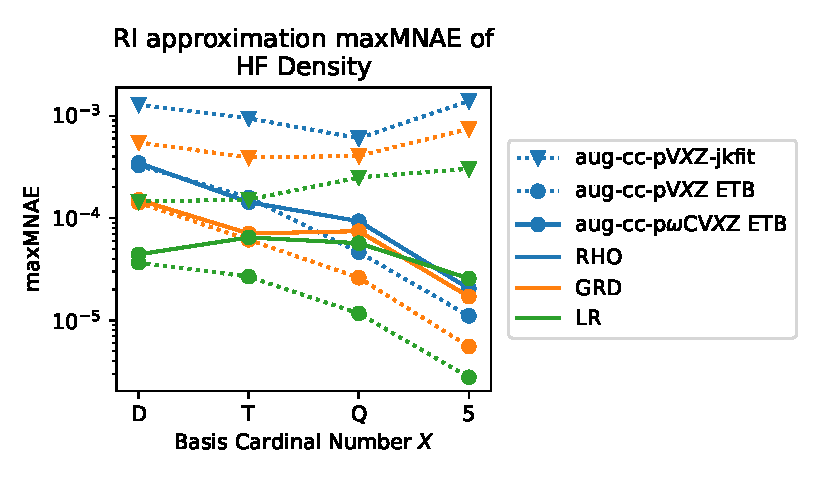
\includegraphics[width=0.7\textwidth]{assets/HF-RI-err.pdf}
\end{figure}

\begin{figure}[h]
  \centering
  \caption{HF 方法 RI 近似下的 meanMNAE 误差。}
  \label{fig.HF-RI-mean}
  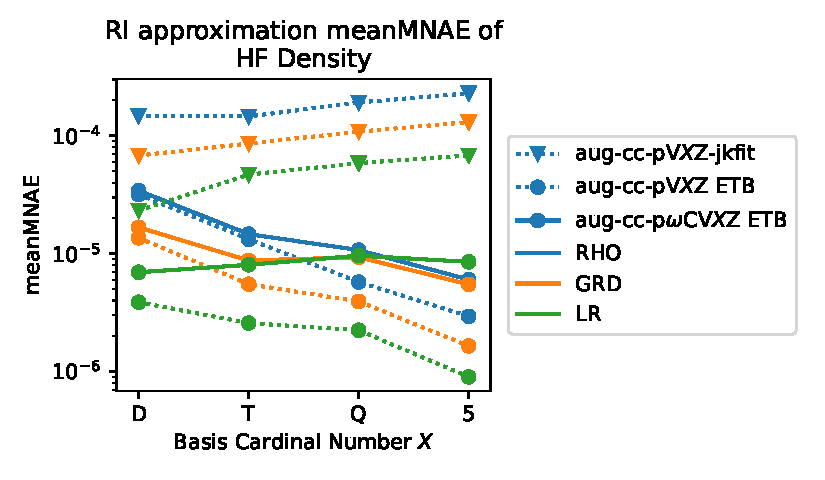
\includegraphics[width=0.7\textwidth]{assets/HF-RI-mean.pdf}
\end{figure}

对于 MP2 方法而言,我们也分别考察了 aug-cc-pV$X$Z-rifit 辅助基\cite{Weigend-Haettig.JCP.2002}、aug-cc-p$\omega$CV$X$Z 辅助基\cite{10.1039/b415208e}与自动辅助基 (ETB)\cite{Stoychev-Neese.JCTC.2017}的表现。这里自洽场部分使用传统 ERI 积分实现,以保证 RI 近似误差仅出现在 MP2 的相关贡献部分。在图 \ref{fig.MP2-RI-err} 与 \ref{fig.MP2-RI-mean} 中,可以看出,采用对 MP2 相关能作优化的 aug-cc-pV$X$Z-rifit 辅助基或 aug-cc-p$\omega$CV$X$Z 辅助基时,密度梯度径向函数 GRD 与二阶梯度径向函数 LR 的误差会较大;对于 GRD,其最大的 MNAE 误差可以达到 0.9;这将会影响泛函或方法在密度径向函数上的评测准确性。相较而言,自动生成辅助基 ETB 方案将给出小于 $10^{-3}$ 的密度径向函数误差;这个误差不会影响测评表现。

\begin{figure}[h]
  \centering
  \caption{MP2 方法相关贡献 RI 近似下的 maxMNAE 误差。}
  \label{fig.MP2-RI-err}
  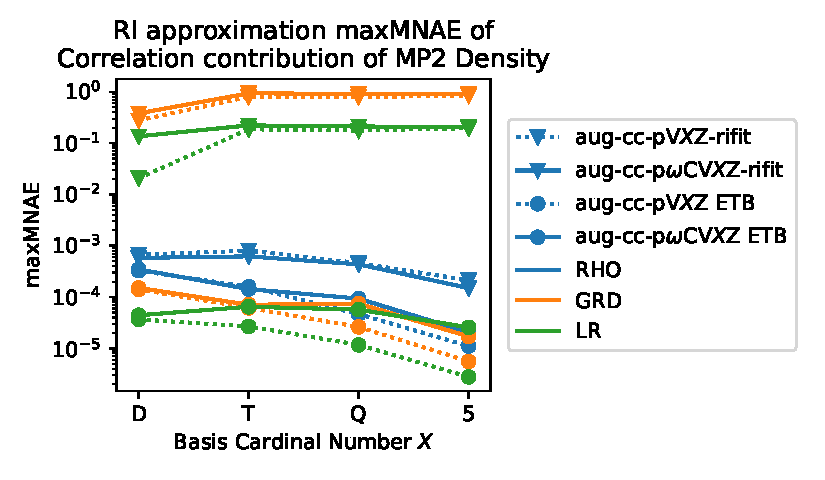
\includegraphics[width=0.7\textwidth]{assets/MP2-RI-err.pdf}
\end{figure}

\begin{figure}[h]
  \centering
  \caption{MP2 方法相关贡献 RI 近似下的 meanMNAE 误差。}
  \label{fig.MP2-RI-mean}
  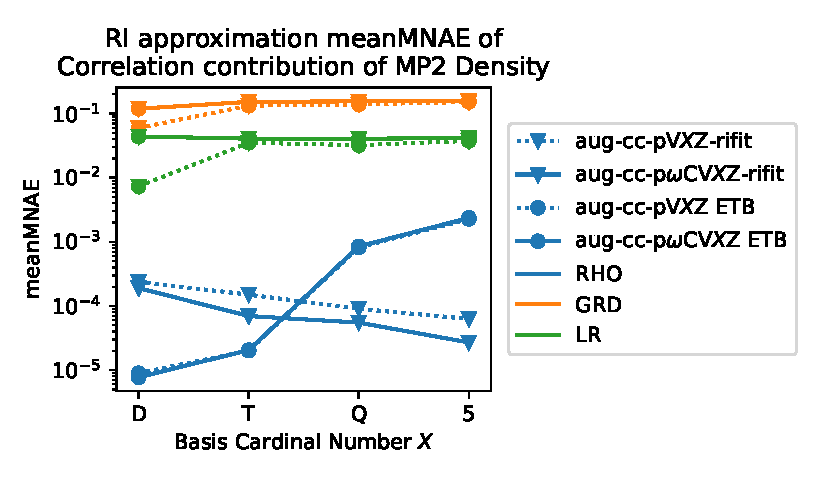
\includegraphics[width=0.7\textwidth]{assets/MP2-RI-mean.pdf}
\end{figure}

从上述简要的分析,我们认为,对自洽场与微扰部分使用自动生成辅助基的 ETB 方案、作 RI 近似,对密度径向函数的影响非常小以至于可以忽略;而采用预制的针对能量计算作优化的辅助基,对于自洽场部分的影响较小、但对微扰部分的影响较大以至于不能忽略。因此,在本工作中,我们统一使用 ETB 方案的辅助基。

\subsubsection{电离能的 RI 近似误差}

我们对 HF 与 MP2 方法的 RI 近似在离子电离能上的误差作简要的评测与分析。评测的方式与上一小节相似。该小节考察的体系是 \ce{Be^+}, \ce{C^2+}, \ce{N^3+}, \ce{O^4+}, \ce{F^5+}, \ce{Ne^6+} 六个离子体系电离两个电子,即 $1s^2 2s^2 \rightarrow 1s^2$ 的电离能。

从图 \ref{fig.HF-RI-eng} 与 \ref{fig.MP2-RI-eng} 可以看出,RI 近似对第二周期元素 $1s^2 2s^2 \rightarrow 1s^2$ 电离能所产生的误差总是小于 $5 \times 10^{-3} \, \text{eV}$;该程度的不影响测评结果。同时,我们注意到,与密度径向函数的情形不同,自动生成辅助基的 ETB 方案在 MP2 相关能计算上的误差,在 $X=\mathrm{T}$ 或更大的基组下,相比于预制辅助基而言要大。

\begin{figure}[h]
    \centering
    \caption{HF 方法 RI 近似下电离能最大误差。}
    \label{fig.HF-RI-eng}
    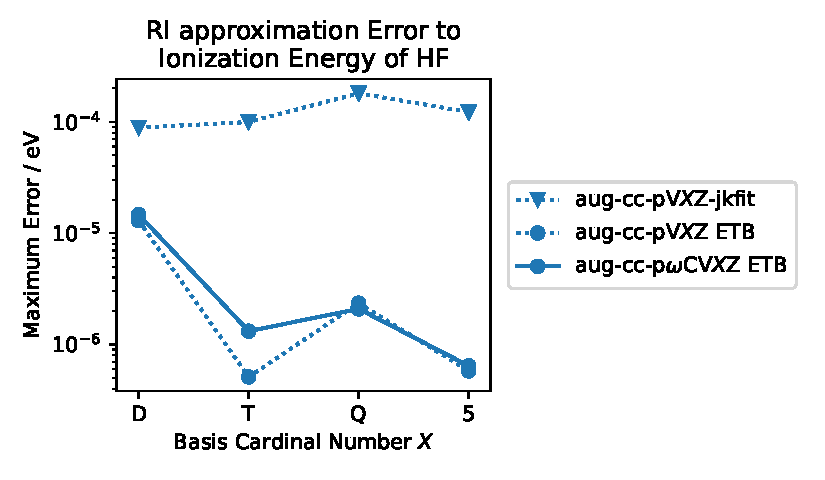
\includegraphics[width=0.7\textwidth]{assets/HF-RI-eng.pdf}
\end{figure}

\begin{figure}[h]
    \centering
    \caption{MP2 方法相关贡献 RI 近似下电离能最大误差。}
    \label{fig.MP2-RI-eng}
    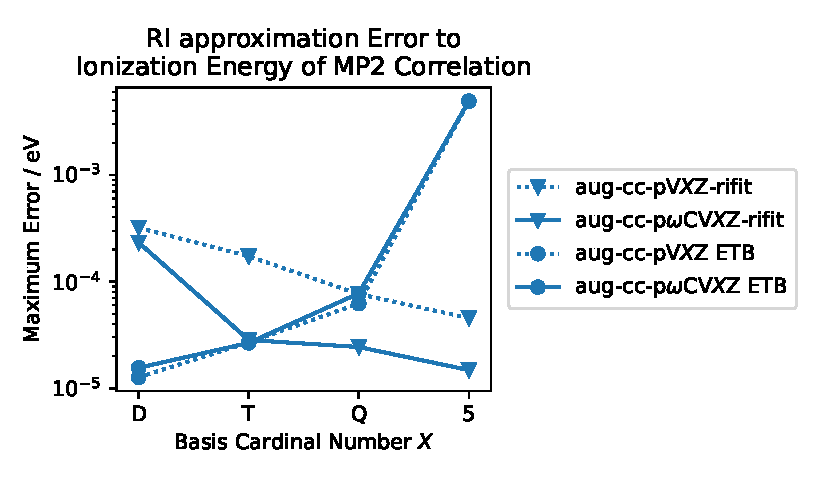
\includegraphics[width=0.7\textwidth]{assets/MP2-RI-eng.pdf}
\end{figure}

我们认为,对于杂化泛函或双杂化泛函,由于其严格交换能和微扰相关能贡献占比小于 100\%,从而 RI 近似对这部分能量或密度所产生的误差,预期不会比完整的 HF 和 MP2 方法更大。因此,我们认为可以在本工作的泛函测评过程中使用 RI 近似。

\newpage

\bibliographystyle{achemso}
\bibliography{../thesis.bib}

\end{document}
